%! Suppress = MissingImport
\chapter{Literature Review}\label{ch:literature-review}
There is a considerable amount of research in the area of resource allocation and task pricing in cloud computing,
in case auction mechanisms are used to deal with competition~\citep{KUMAR2017234,Zhang2017,Du2019,Bi2019}.
Section~\ref{sec:resource-allocation-and-auctions-in-cloud-computing} presents the different approaches to resource
allocation and pricing mechanisms in cloud computing and MEC.

The proposed solution of the project (presented in chapter~\ref{ch:proposed-solution-to-problem}) uses a form of
machine learning, called Reinforcement Learning. Section~\ref{sec:reinforcement-learning} explains the algorithms
implemented from Q learning and policy gradient research.

\section{Resource allocation and auctions in Cloud Computing}\label{sec:resource-allocation-and-auctions-in-cloud-computing}
A majority of approaches taken for task pricing and resource allocation in cloud computing uses a fixed resource
allocation mechanism, such that each user requests a fixed amount of resources from a server for a task. However this
mechanism, as previously explained, provides no control over the quantity of resource allocated to a task for a server,
only the task price. As a result, a majority of approaches don't consider the server may manage resource allocation,
rather research has focused on designing efficient and strategyproof auction mechanisms.
% TODO on pricing on cloud computing
% Actuall present the different approaches to auction mechanisms in cloud computing
% A survey of these approaches for double auction mechanism in cloud computing is outlined by~\cite{KUMAR2017234},
% \citep{KUMAR2017234,Zhang2017,Du2019,Bi2019}.

Research by~\cite{vaji_infocom}, considers the placement of code/data needed to run specific tasks as a the scheduling
of tasks to different edge server as an alternative method to increase the flexible when running tasks. The goal is to
maximise the expected rate of completed tasks over time with the assumption that data/code can be shared.
% TODO read the paper and add another two sentences explaining the work

Previous work by this author in~\cite{FlexibleResourceAllocation} proposed the novel resource allocation mechanism and
optimisation problem that this project works to expand. The paper presents three mechanism for the optimisation problem,
one to maximise the social welfare and two auction mechanisms. The Greedy algorithm presented allows for quick
approximation of a solution through the use of several heuristics in order to maximise the social welfare. Results
found that the algorithm achieved over 90\% of the optimal solution given certain heuristics compared to fixed
resource allocation solution that achieved 70\%. The algorithm has polynomial time complexity with a lower bound of
$\frac{1}{n}$ however in practice achieves significantly better results.

The work also presented a novel decentralised iterative auction mechanism developed using the VCG
principle~\citep{vickrey, Clarke, groves} in order to iterative increase a task's price. As a result, a task doesn't
reveal its private task value that is viewed as advantageous for users who wish to not reveal how important their task
is to them, particularly in tactical network. The auction mechanism achieves over 90\% of the optimal solution due to
iteratively solving of a specialised server optimisation problem. The third algorithm is an implementation of a single
parameter auction~\citep{nisan2007algorithmic_critical_value} using the greedy algorithm to find the critical value for
each task. Using the greedy algorithm with a monotonic value density function means the auction is incentive compatible
and inherits the social welfare performance and polynomial time complexity of the greedy mechanism.

\section{Reinforcement learning}\label{sec:reinforcement-learning}
Computer scientists have always been interested in comparing computers against humans~\citep{turing1950computing} and a
key characters of humans is the ability to learn from experience. For computers this ability is complex to perform with
researchers finding a variety of ways for computers to do this. These methods are broadly grouped into three categories:
supervised, unsupervised and reinforcement learning. Supervised learning uses inputs that mapped to outputs, an example
is image classifications. While unsupervised learning doesn't have a known output for inputs to be mapped to, instead
these algorithms tries to find links between similar data, for example data clustering.

However both of these techniques are not applicable for case where agents must interact with an environment making a
series of actions that result in rewards over time. Algorithms designed for these problems fall into the category of
Reinforcement Learning that aim to maximise the agent rewards. These algorithms utilise environments that can be
formulated as a Markov Decision Process~\citep{Bel}. Because of the number of application for reinforcement learning,
it is a rapidly growing field of research within AI particularly in the last 5 years.

% Figure reinforcement learning model

\begin{figure}[h]
    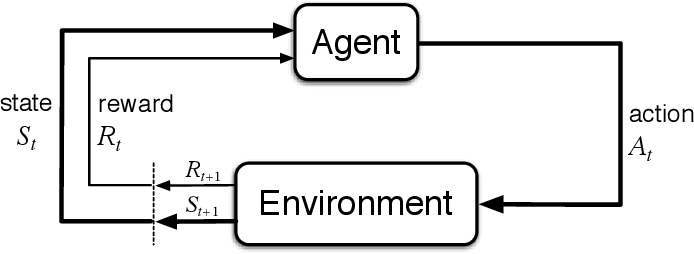
\includegraphics[width=10cm]{figures/reinforcement_learning.png}
    \caption{Reinforcement learning model (Source: ~\cite{Sutton1998})}
    \label{fig:reinforcement_learning}
\end{figure}


Q-learning algorithm~\cite{watkins1992q-learning} is a learning method used for estimating the action-value function,
one of the bases on for modern reinforcement learning. As the series of actions can be formed into a tree of
actions, an agent is interested in which actions will result in the largest reward in the future. This is formulated
as in equation~\eqref{eq:q_learning}.

\begin{align}
    Q(s_t, a_t) = E[R_{t+1} + \gamma R_{t+2} + \gamma^2 R_{t+2} + \cdots ] \label{eq:q_value} \\
    Q(s_t, a_t) = Q(s_t, a_t) + \alpha \cdot (r_t + \gamma \cdot \text{max}_a Q(s_{t+1} , a) - Q(s_t, a_t) ) \label{eq:q_learning} \\
\end{align}

However the curse of dimensionally was found to be a major problem as to use Q learning required
forming a table of state-actions in order to calculate and as the number of dimensions increase, the number of
state-actions will increase exponentially. Therefore making the method impractical for problem that had large state
space. Therefore use of a function approximate is used to circumvent this problem, traditionally done using a neural
network. Work by~\cite{atari} using a deep convolution neural network was able to achieve state of the art in six of seven
games tried on atari with three of these scores being superhuman. This work was followed up by~\cite{mnih2015humanlevel}
and found that with no modifications to the hyperparameters, neural network and training method; state of the art results were
achieved in almost all 49 atari games and superhuman results in 29 of these games. Additional heuristics have been
proposed for deep Q learning: double DQN~\citep{doubledqn}, prioritized experience replay~\citep{prioritizedexperiencereplay},
dueling network architecture~\citep{duelingdqn}, multi-step bootstrap targets~\citep{multi-step-dqn, Sutton1998},
A3C~\cite{A3C}, distributional Q-learning~\citep{distributional_dqn} and noisy DQN~\citep{noisy_dqn}. These methods were
combined to together~\cite{rainbow}, called rainbow DQN, achieving over 200\% of the original DQN algorithm and over
50\% than any optimisation on its own in a quarter of the observations.

\begin{figure}[h]
    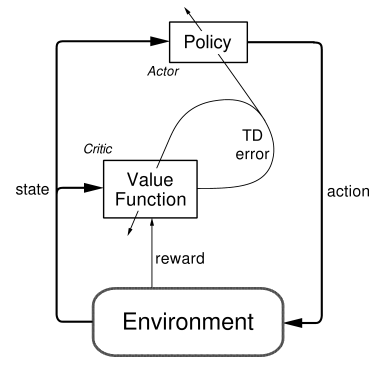
\includegraphics[width=10cm]{figures/actor-critic.png}
    \caption{Actor Critic model (Source: ~\cite{Sutton1998})}
    \label{fig:actor-critic-model}
\end{figure}

Using the base of Q-learning, policy gradient~\ref{fig:actor-critic-model} separate the action selection policy to the
q-value policy. In Q-learning, the selection the action is based on the maximum Q-value of the actions however policy
gradient separates. This has the advantages of being able to deal with both discrete and continuous action spaces where
Q-learning can only deal with discrete action space. Also the learning method doesn't require $\epsilon$-greedy action
selection that can for Q-learning cause the resulting policy to differ from the optimal policy. Therefore policy
gradient has been used to master the game of Go~\citep{silver2017mastering} and achieve top 1\% in
Dota 2~\citep{OpenAI_dota} and Starcraft 2~\citep{starcraft2}.